\documentclass{article}
\usepackage{graphicx} % Required for inserting images
\usepackage{hyperref}
\usepackage[a4paper, margin=0.8in]{geometry}
\usepackage{listings}
\usepackage{fancyhdr} 
\usepackage{svg}
\usepackage{tikz}
\usepackage{color}
\usepackage{tabularx}
\usepackage{longtable}
\usepackage{pdflscape}

\hypersetup{
	colorlinks=true, %set true if you want colored links
	linktoc=all,     %set to all if you want both sections and subsections linked
	linkcolor=black,  %choose some color if you want links to stand out
	citecolor=gray,  %color for referencing bibliography
}

\AfterPreamble{\hypersetup{ %metadata for pdf generation
  pdfauthor={Luca Salmoiraghi, Tobia Grimaldi, Dong Hua Zhu},
  pdftitle={Astralog-HPC - Requirement analysis and design document},
  pdfsubject={Software engineering, Requirement Analysis}
}}

% Impostazioni fancyhead e fancyfoot
\pagestyle{fancy}
\renewcommand{\sectionmark}[1]{
	\markboth{\thesection\quad #1}{}}
\fancyhead{}
\fancyhead[L]{\nouppercase{\leftmark}}
\fancyfoot{}
\fancyfoot[C]{\thepage}

\fancypagestyle{landscapepage}{
    \fancyhf{}                    % svuota header e footer
    \fancyfoot[C]{}       % numero pagina al centro
    \renewcommand{\headrulewidth}{0pt}
    \renewcommand{\footrulewidth}{0pt}
}

\newcommand{\tablerefer}[1]{%
    \hyperref[#1_top]{Table \ref*{#1}}%
}

\newcommand{\figurerefer}[1]{%
    \hyperref[#1]{Figure \ref*{#1}}%
}

\input{Configuration_files/json_lstlisting} %stlistng json definition

%\title{Astralog-HPC} %TODO: BETTER TITLE
%\author{Luca Salmoiraghi, Tobia Grimaldi, Dong Hua Zhu}
%\date{April 2026} By commenting this line, the date of the last modification is automatically inserted
%TODO: The initial page should include project title, version of the document, names and release date (maybe versioning as well?)
% rivedo tutto più tardi se ho tempo ma penso che la Di Nitto si riferisse più al versioning del software che del documento.

\begin{document}

%\maketitle
\definecolor{bluePoli}{cmyk}{0.4,0.1,0,0.4}
\begin{titlepage}
    \begin{tikzpicture}[remember picture, overlay]
        % background
        \def\tilesize{2cm} 
                
                % Start tiling from the bottom-left to the top-right
                \foreach \x in {0, 1, ..., 15} {% 
                    \foreach \y in {0, 1, ..., 20} {%
                        \node[opacity=0.05, inner sep=0pt, outer sep = 0pt, anchor=south west] 
                        at ([xshift=\x*\tilesize, yshift=\y*\tilesize]current page.south west) {
                            
\includegraphics[width=\tilesize, height=\tilesize]{images/line-in-motion.pdf}
                        };
                    }
                }
        % The vertical accent bar
        \fill[bluePoli] (current page.north west) ++(1.5cm,0) rectangle ++(0.3cm,-\paperheight);
    \end{tikzpicture}

    \hspace{2cm}
    \begin{minipage}{0.8\textwidth}
        \vspace{2cm}
        \sffamily
        {\Large \color{gray} Requirement Analysis and Design Document} \\[0.25cm]

        {\Huge \textbf{Astralog-HPC}} \\[0.1cm]

        {\large \textit{High-Performance Computing Space Mission Logging System}}
        
        \vspace{3cm}
        
        \textbf{PREPARED BY} \\
        Luca Salmoiraghi \\
        Tobia Grimaldi \\
        Dong Hua Zhu
        
        \vspace{2cm}
        
        \textbf{PROJECT SCOPE} \\
        This document outlines the domain assumptios, functional and non-functional requirements, 
        system architecture, and design patterns for the Astralog-HPC environment.
        
        \vspace{1cm}

        \textbf{DATE OF CREATION} \\
        April 4, 2026
        
        \textbf{LAST UPDATED ON} \\
        \today
    \end{minipage}
\end{titlepage}
\clearpage
\tableofcontents
\clearpage

\section{Introduction to the project and project goals}

\subsection{Overview}

Modern space missions produce a large and uninterrupted flow of telemetry data. To safeguard spacecraft, the development of \textbf{AstraLog-HPC} is required. AstraLog-HPC is a software tool designed for anomaly detection in onboard systems. It ingests data streaming from spacecraft sensors within each system and subsystem, filters systematically invalid packets and applies monitoring rules based both on the absolute value of incoming data as well as on their changes over time and their interdependencies.
AstraLog-HPC is designed to produce both a summary of non-anomalous telemetry and a log of detected errors for mission personnel, enabling them to prioritise safety decisions and plan subsequent actions that safeguard mission success.
Additionally, the system must support operation both onboard, on embedded systems for real-time ingestion and high-priority anomaly detection, and on-ground in data centres, for high-volume, lower-priority data analysis. 

\medskip
This project aims to put into practice what was learned from the first part of the Software Engineering for HPC course. In particular, this document covers principles of requirement engineering and architectural design.  

\subsection{Goals}

%The main function of the software is to monitor the continuous data that come from different sensors placed on various subsystems, filter out for syntactically invalid packets, and accumulate valid packets into a local batch file; 
% the filtering process is triggered once the batch reaches the size specified.
% filtering process regards discarding invalid packets, so it happens on the fly (or
% at least this is what I get). Batch size check refers to the application of monitoring rules.
%when the batch reaches a specified size, the system applies four types of rules to all collected valid data.
%Luca: this seems quite redundant, espacially since everything is welle detailed in the next bullet point.
The primary goals of AstraLog-HPC can be organised into three categories: 

% I am not sure if to specify the monitoring rules here in the 'Goals' paragraph.
% I would focus more on the goals of the project in general (Luca: yeah, I totally agree, we might consider adding a separete section if necessary)
%\medskip
%Thus, the primary goal is to implement a robust monitoring system capable of evaluating data against the %following logic:
%\begin{itemize}
%    \item \textbf{Simple Rule (Absolute Threshold)}: checks if a value exceeds a fixed threshold at a given time
%    \item \textbf{Step Difference Rule (Relative Variation)}: checks the difference between the current measurement and the previous measurement are equally spaced
%    \item \textbf{Stateful Rule (Measurement Persistence)}: an anomaly is triggered only if a specific simple condition persists uninterrrupted for a given number of consecutive measurements
%    \item \textbf{Logical Correlation Rules}: Combines the Boolean outcomes of the other evaluated rules at the same tamestamp using standard logical operators
%\end{itemize}

% my version
\begin{itemize}
    \item \textbf{Robust Data Ingestion and Cleansing}: The system must be capable of receiving a continuous stream of JSON telemetry data from various sensors across different subsystems. It shall detect and discard invalid packets (further discussed in Table \ref{tab:corruption_cases}) and noisy measurements commonly occurring in real-time space communication.
    \item \textbf{Collect Data into Batches for Processing}: Valid packets shall be accumulated into a local batch file. When a batch reaches a specified size and/or enough time from the last sent batch is elapsed, the system triggers the Anomaly Detection phase.
    \item \textbf{Anomaly Detection and Rules Application}: The core goal of the system is to analyse valid packets of data and detect anomalies according to four different types of rules (further discussed in Table \ref{tab:monitoring_rules}).
\end{itemize}
% I know it is not perfect but maybe these are some examples of more general goals of the system. I guess the specifications about monitoring rules and corruption cases will be further described in next sections.

\clearpage
\section{Requirement analysis}
\subsection{Relevant human and non-human actors}
This section identifies the external entities that interact with AstraLog-HPC. Actors are categorized based on whether they directly interact with the system (Primary) or provide support to achieve a goal (Secondary).\\
\tablerefer{tab:actors} provides and overview of identifiable actors. 
\begin{table}[h!]
\label{tab:actors_top}
\centering
\begin{tabularx}{\textwidth}{|l|l|X|}
\hline
\textbf{Actor} & \textbf{Category} & \textbf{Responsibility} \\ \hline
\textbf{Ground Station Operator} & Primary (Human) & Responsible for spacecraft configuration and health monitoring. They define the environment via configuration files  and serve as the primary consumer of system alerts. \\ \hline
\textbf{MQTT Broker} & Primary (Non-Human) & Acts as the central message intermediary. The system interacts with the broker subscribing on a topic in order to receive the stream of packets. \\ \hline
\textbf{Sensors} & Secondary (Non-Human) & Hardware or software components on the aircraft that function as data producers. They capture telemetry data, encapsulate it into JSON packets, and publish it to the Broker. \\ \hline
\textbf{SLURM Job Scheduler} & Secondary (Non-Human) & Enables access to the HPC cluster. Responsible for allocating resources and scheduling the deployment of system components. \\ \hline
%TODO (Luca): I think an additional actor (e.g. a Monitoring GUI or something like that) should be included, just to give a reason for producing valid_data.csv
\end{tabularx}
\caption{AstraLog-HPC System Actors and Responsibilities}
\label{tab:actors}
\end{table}

\subsubsection{Human Actors}
The main human actor that interacts with the system is: 
\begin{itemize}
    \item \textbf{Ground Station Operator (Primary):} This actor is responsible for the configuration and health monitoring of the spacecraft. The operator defines the environment by providing the configuration files which specify the rules to be aware of and the sensors sending data. Furthermore, operators serve as the primary consumer of system alerts, accessing \verb|alarms.log| to make high-level safety decisions regarding aircraft subsystems.
\end{itemize}
\subsubsection{Non-Human Actors}
Main non human actors that interact with the system are:
\begin{itemize}
    \item \textbf{MQTT Broker (Primary):} First component the system interacts with in order to receive the packets stream from spacecraft. AstraLog-HPC establishes a permanent connection with the Broker subscribing to the topic \verb|esa/astralog/telemetry|.
    \item \textbf{Sensors (Secondary):} Hardware or Software entities that reside on the spacecraft. They are responsible for all the measurements regarding the spacecraft status (e.g. temperature, voltage, current, pressure). They do not directly interact with the AstraLog-HPC environment and are therefore reported here only for the sake of completeness.  
    \item \textbf{SLURM Job Scheduler (Secondary):} This entity manages access to an HPC cluster. It is responsible for allocating resources and scheduling the deployment of AstraLog-HPC components when the system runs in ground-based, high-volume processing mode.
\end{itemize}
\subsection{Use cases}
This section describes the main use cases of the AstraLog-HPC system. The use cases define the functionalities provided by the application as well as the interactions between them and the actors that interact with the system.
These interactions are visualized in the use case diagram below (Figure \ref{fig:use_case}), while \tablerefer{tab:use_case_actors} provides a terse overview of the role of each actor in each use case.
\subsubsection*{Description of the Presented Use Cases}
% I see that usually professor uses the camel case format or whatever it is. I dont think it is the best but for the moment I will stick with it
\begin{itemize}
    \item \textbf{IngestData: }The system receives a continuous stream of JSON packets from the aircraft sensors. First  This process includes the mandatory validation of packet syntax and structure.
    \item \textbf{DetectCorruptionCases: }Triggered during ingestion, the system filters out invalid packets. It specifically identifies malformed JSON, schema errors (missing mandatory fields), and type errors (invalid data formats).
    % eventual specilization for this use case
    \item \textbf{MonitorSystemStatus: }The system aggregates valid packets in batches and later evaluates the state of the spacecraft given a set of monitoring rules in \verb|rules.json|.
\end{itemize}
\subsubsection*{Conditional Outcomes}
The following use cases extend \textit{MonitorSystemStatus}, defining the behaviour of the system if an aggregated batch respects or not one or more of the monitoring rules defined in \verb|rules.json|:
\begin{itemize}
    \item \textbf{LogNominalState: }If a data batch is evaluated and no violation is detected, the system appends an entry to the \verb|valid_data.csv| file.
    \item \textbf{ReportAlarm: }If one or more rule is evaluated to TRUE, the incorrect state of the system is reported with an alarm in the \verb|alarm.log|.
\end{itemize}
\begin{figure}[htbp]
    \centering
    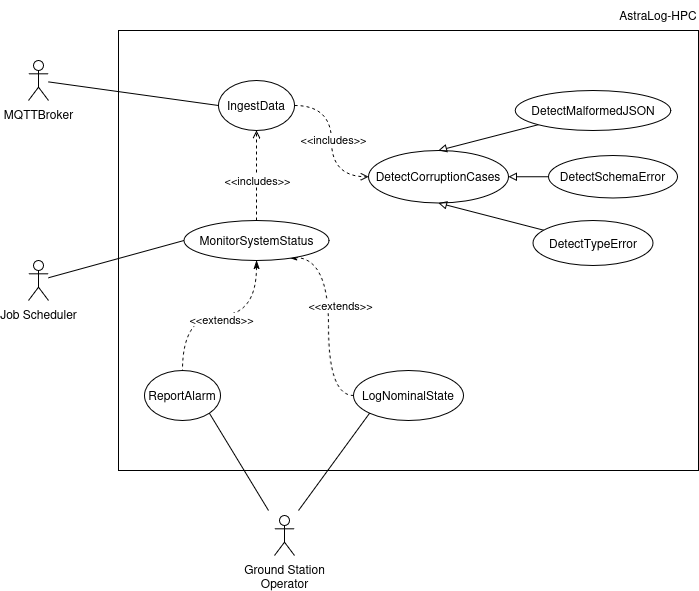
\includegraphics[width=0.70\textwidth]{images/usecases_diag.png}
    \caption{AstraLog-HPC Use Case Diagram}
    \label{fig:use_case}
\end{figure}
\begin{table}[h]
    \centering
    \label{tab:use_case_actors_top}
    \begin{tabularx}{\textwidth}{|X|X|X|}
        \hline
        \textbf{Use Case} & \textbf{Primary Actor} & \textbf{Secondary Actor} \\
        \hline
        IngestData & MQTT Broker & Sensors \\
        \hline
        DetectInvalidPackets & (internal) & None \\
        \hline
        MonitorSystemStatus & Ground Station Operator & SLURM (for HPC mode) \\
        \hline
        LogNominalState & Ground Station Operator & None \\
        \hline
        ReportAlarm & Ground Station Operator & None \\
        \hline
    \end{tabularx}
    \caption{Use Case to Actor Mapping}
    \label{tab:use_case_actors}
\end{table}
% OK so far the use case diagram is pretty plain but I guess we will have time to update it,
% Of course we can downlaod files from the image folder and load it on draw.io so that we can 
% modify it on the fly.
\subsection{Domain assumptions}
This section documents the domain-specific assumptions underlying and justifying the design decisions of AstraLog-HPC. These assumptions are accepted as true and the software is developed according to these premises. The correct behaviour of the system is not guaranteed outside of these assumptions.\\
Specifically, the system assumes the following:
\begin{itemize}
    \item The spacecraft systems and subsystems operate over a unified synchronous system clock.
    \item All measurements across all sensors are equally spaced in time and perfectly aligned (that is, all sensors produce data for the entire duration of the mission, no failures of sensors). Each sensor publishes on a specific topic with a 1Hz rate.
    \item Each spacecraft contains multiple sensors types, each eventually available in multiple instances. The type of sensor is determined by the particular quantity which is measured. 
    \item The specific type and number of sensors to be managed are available in a configuration file called \verb|sensors.yaml|, which means the number of sensors is assumed to remain constant throughout the entire operation of the system.
    \item Each sensor continuously produces data, which is published to the MQTT Broker in the form of a standardised \verb|.json| package with the following example structure:
\begin{lstlisting}[language = json]
    {
        "timestamp": "2025-11-15T12:00:00Z",
        "sensor_id": "TEMP-01",
        "value": 25.5,
        "priority": "HIGH"
    }
\end{lstlisting}
    \item Data transmission is often noisy, which means received packets could be invalid, having missing data or wrong format.
    \item The data collected in a certain clock cycle, corresponds to the $n$-th measurement of each sensor. This means all the packets received together belong to measurements happened at the same time.
    \item Monitoring rules are available in a \verb|rules.json| file, accessible by AstraLog-HPC.
    \item Each monitoring rule in the previously mentioned \verb|rules.json| file belongs to one of four types of rules (\tablerefer{tab:monitoring_rules}) Moreover, each monitoring rule has a unique ID. 
    \item Monitoring rules check is performed just after the system collects a batch size of valid packets from the Broker.
    \item Eventually, monitoring rules are characterized by a \textit{PRIORITY} attribute. Rules with an higher priority parameter are evaluated before the others among the same type. % strange it is reported like this in the paper but ok, maybe give your opinion to be sure
\end{itemize}

\subsection{Requirements}
This section specifies the functional and non-functional requirements for AstraLog-HPC. Functional requirements specify what the system must do, while non-functional requirements define quality constraints and shape how the system performs its actions.
\subsubsection{Functional requirements}
The following functional requirements describe the specific behaviours, tasks and operations that AstraLog-HPC must support:
%TODO: AI suggested giving a label to these requirements, to ensure tracebility. Seems good to me, to me aswell but no idea how to do it
\begin{itemize}
    \item The system should receive the streamed data in the format of JSON packets by establishing a persistent subscription to the MQTT Broker on the \verb|esa/astralog/telemetry| topic.
    \item The system should filter invalid packets. A packet is considered invalid whenever one of the following corruption cases verifies (\tablerefer{tab:corruption_cases}):
    \begin{table}[h!]
    \label{tab:corruption_cases_top}
    \centering
    \begin{tabularx}{\textwidth}{|l|X|}
    \hline
    \textbf{Error Type} & \textbf{Description} \\ \hline
    \textbf{Malformed JSON} & Transmitted packet has an invalid JSON syntax. \\ \hline
    \textbf{Schema Errors} & A packet is missing mandatory fields required for processing. \\ \hline
    \textbf{Type Errors} & A sensor is sending data of an invalid or unexpected data type. \\ \hline
    \end{tabularx}
    \caption{Definition of Packet Corruption Cases}
    \label{tab:corruption_cases}
    \end{table}
    \item The system should accumulate the valid packets in a batch file to be used to analyse data according to the monitoring rules
    (\tablerefer{tab:monitoring_rules}):
    \begin{table}[!h]
    \label{tab:monitoring_rules_top}
    \centering
    \begin{tabularx}{\textwidth}{|l|l|X|}
    \hline
    \textbf{Rule Type} & \textbf{Evaluation Logic} & \textbf{Trigger Condition} \\ \hline
    \textbf{Simple Rule} & Absolute Threshold & Evaluates if a sensor measurement crosses a fixed threshold at a specific point in time. \\ \hline
    \textbf{Step Difference} & Relative Variation & Evaluates the difference between the current measurement and the immediately preceding one. \\ \hline
    \textbf{Stateful Rule} & Persistence & Triggers only when a condition is continuously violated over a defined number of consecutive measurements. \\ \hline
    \textbf{Logical Correlation} & Boolean Combination & Combines outcomes of multiple rules at the same timestamp using operators like AND or OR. \\ \hline
    \end{tabularx}
    \caption{AstraLog-HPC Monitoring Rule Definitions}
    \label{tab:monitoring_rules}
    \end{table}
\end{itemize}
In particular, after having filtered the invalid packets and sent them to the ground station, the system should operate in the following way: 
\begin{itemize}
    \item if no rules are violated, the system should append a single aggregated line to the output file \verb|valid_data.csv| following the format: 
\begin{lstlisting}[language = json]
    TIMESTAMP;NOMINAL;[SENSOR_1]:[VALUE_1]|[SENSOR_2]:[VALUE_2]|...
\end{lstlisting}
An example is provided: 
\begin{lstlisting}[language = json]
    2025-11-15T12:00:00Z;NOMINAL;TEMP-01:25.5|PRES-01:101.3|VOLT-
    MAIN:24.1
\end{lstlisting}
    \item if one or more rules are violated, nothing is written to \verb|valid_data.csv|, while each violated rule is reported in the output file \verb|alarms.log| following the format: 
\begin{lstlisting}[language = json]   
    TIMESTAMP;RULE_ID;PRIORITY;VIOLATED_SENSOR(S);CURRENT_VALUE(S)
\end{lstlisting}
Two examples are provided: 
\begin{lstlisting}[language = json]
    2025-11-15T12:00:05Z;R1;MEDIUM;TEMP-01;51.2
    2025-11-15T12:00:05Z;R4;HIGH;TEMP-01,PRES-01;51.2,98.0
\end{lstlisting}
\end{itemize}
\subsubsection{Non-functional requirements}
The following non-functional requirements define the quality characteristics and constraints of AstraLog-HPC, including performance, reliability, scalability, and operational boundaries:
\begin{itemize}
    \item In order to handle the continuous flow of data from a spacecraft, AstraLog-HPC must be optimised for batch processing to handle high-throughput sensor data efficiently. 
    \item The system should maintain data consistency by subscribing to an \textit{HiveMQ MQTT} Broker. This means that the entire telemetry must be collected on a topic and maintained safe even in conditions of network instability.
    \item The system must be capable of executing with a consistent behaviour in multiple environments, from classical to virtual machines and HPC clusters.
    \item The deployed architecture must allow access to an HPC cluster through a SLURM Job Scheduler.
    \item To exploit the HPC cluster capabilities, the system should be capable of optimising data ingestion aggregating JSON packets into batches.
    \item The system should support parallel evaluation of rule across data batches to fully exploit the capabilities of an HPC environment.
    \item Given the highly critical field of application of the software, reliability and stability are crucial characteristics the system should pursue.
    \item The system must produce coherent output text in order to permit verifiability of software and allowing to correctly perform safety checks on the implementation.
    \item The software structure must be clearly defined and documented, allowing for the easy addition of new rule types and eventual newly defined behaviours.
\end{itemize}

\clearpage
\section{Design}
\subsection{General description of the architecture}

The AstraLog software base relies on a \textbf{Component-Based Architecture}. Each component of the system performs a specific, well-defined job and interacts with the others exclusively through interfaces, ensuring reliability, scalability and maintainability.

\medskip

The system is comprised of the following components: 
\begin{itemize}
    \item \textbf{DataIngestor}: handles the stream of data provided by the Broker and imports it in the Astralog-HPC system; It also filters out syntactically invalid packets, given the corruption cases already defined (\tablerefer{tab:corruption_cases}).
    % \item \textbf{InvalidPacketsFilter}: filters out syntactically invalid packets; %[Mike: having a dedicated component for the filtering isn't rendudant? We can put the filtering logic within the Data Injector in order to reduce latency] [Tob: si sono d'accordo con Mike. Tralaltro il filter non conserva uno stato ma decide semplicemente se il pacchetto è corretto o no. In più ci rende l'implementazione dell'Ingestor più semplice]
    \item \textbf{BatchAccumulator}: accumulates filtered (hence valid) packets in a local batch file for further processing, it must accumulate up to a specified batch file dimension;
    \item \textbf{RuleLoader}: reads and provides access to static configurations and rules, specifically monitoring rules from \verb|rules.json|. Moreover, it handles the reordering of these rules given a \textit{PRIORITY} parameter;
    \item \textbf{ThreadSafeBuffer}: collects the complete batches accumulated in the Batch Accumulator and appends them in a queue structure;
    \item \textbf{RuleEngine}: pops the first element from the ThreadSafeBuffer's queue and applies the previously loaded rules to the batch according to a priority value (low, medium, high);
    \item \textbf{MeasDatabase:} database where we store previous measurements associated to each sensor. Specifically used to evaluate step-difference and stateful rules;
    \item \textbf{OutputDispatcher}: directs the evaluation results to the correct files. If no rules are violated, the batch files is appended to \verb|valid_data.csv|, otherwise nothing is written to \verb|valid_data.csv|, while all the violated rules are reported on \verb|alarms.log|.
\end{itemize}

Their mutual relation is expressed by the following component diagram (Figure \ref{fig:component_diag}): 
\begin{figure}[htbp]
    \centering
    \label{fig:component_diag}
    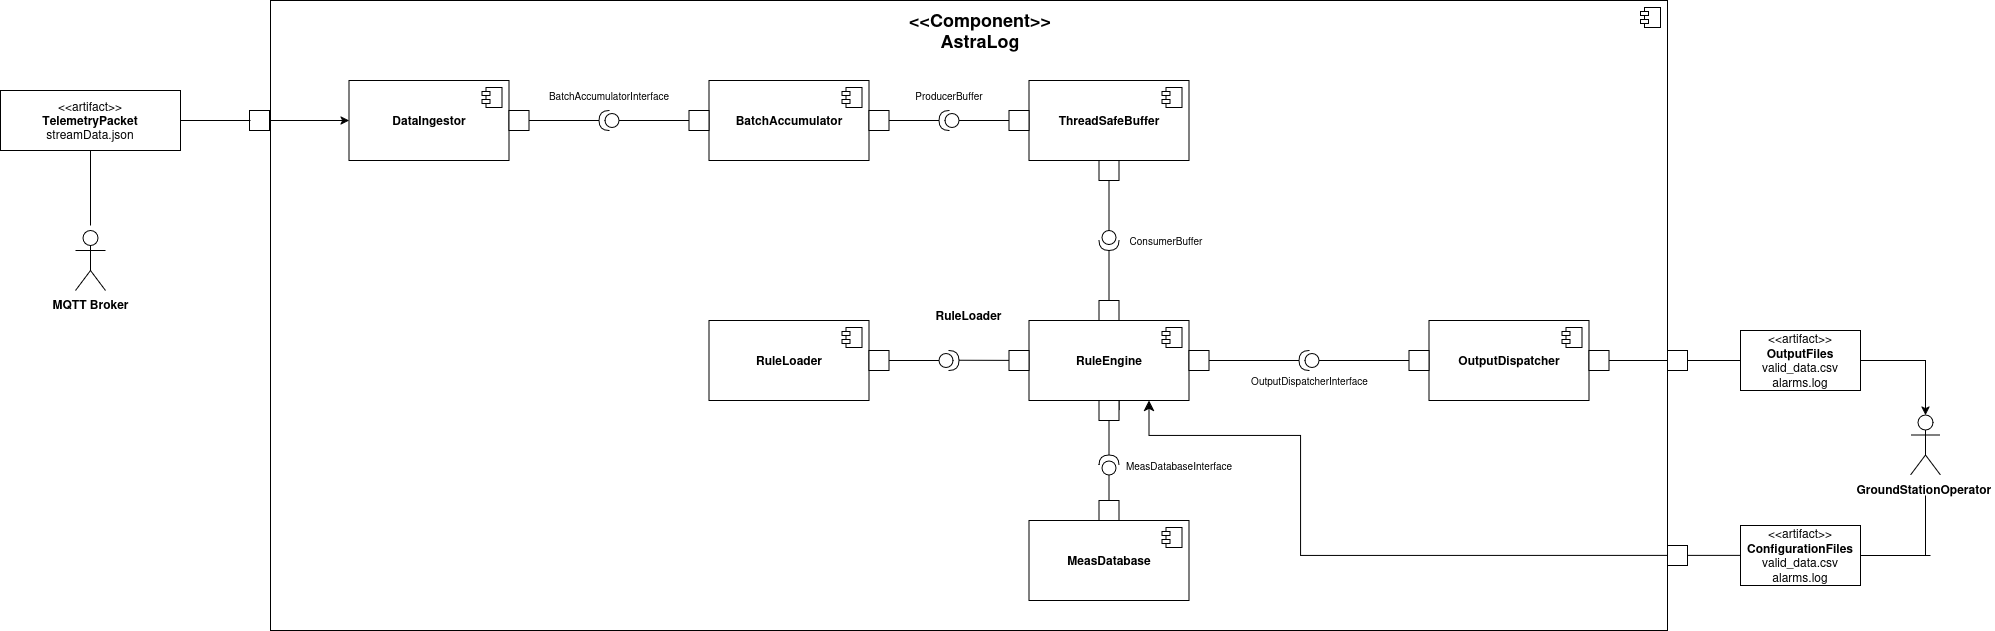
\includegraphics[width=\textwidth]{images/ComponentDiagram/ComponentDiagram.drawio.png}
    \caption{AstraLog-HPC: Component Diagram}
    \label{fig:component_diag}
\end{figure}

\subsubsection{Pipeline}

The data flow follows a clear pipeline: DataIngestor receives raw stream data from external sources, filters out malformed JSON entries, and parses the valid ones. The parsed data is forwarded to BatchAccumulator, which buffers incoming records until a configured batch size is reached, then pushes the batch into ThreadSafeBuffer. The RuleEngine consumes batches from the buffer, applies the configured rules, and sends a result summary to OutputDispatcher.

\subsubsection{Design patterns}

To structure the pipeline, three design patterns are employed:

\begin{itemize}
    \item \textbf{Producer-Consumer:} BatchAccumulator acts as the producer, pushing batches into the ThreadSafeBuffer queue, while RuleEngine acts as the consumer, extracting and processing them. This decouples data accumulation from rule processing and ensures thread-safe communication between the two;
    \item \textbf{Strategy:} RuleEngine acts as the context and operates on a BaseRule abstract class. Each concrete rule is a subclass of BaseRule, allowing different rule implementations to be selected and applied interchangeably at runtime without modifying the engine logic;
    \item \textbf{Centralised Rule Creation:} RuleLoader is responsible for instantiating the correct BaseRule subclass based on the rule configuration, centralising and decoupling object creation from the rest of the system.
\end{itemize}

\begin{landscape}
\subsection{Class Diagram}
\thispagestyle{landscapepage}
\begin{figure}[h]
    \centering
    \includesvg[width=1.5\textheight]{images/ClassDiagram/ClassDiagram.svg}
    \caption{AstraLog-HPC: Class Diagram}
    \label{fig:class_diag}
\end{figure}
\end{landscape}

\subsubsection{Simplifications and variations}
The RuleLoader component was originally conceived following the Factory Method pattern, where separate creator subclasses would each be responsible for instantiating a specific BaseRule subtype.

\medskip

In the actual implementation, this was simplified into a Simple Factory approach: a single loadRules method dispatches object creation through an if/elseif chain based on the rule "type" field, with dedicated private parsing methods (parseSimpleRule, parseStepDifferenceRule, parseStatefulRule, parseLogicalCorrelationRule) for each concrete type. While this does not constitute a formal GoF pattern, it preserves the core intent of centralising and decoupling rule instantiation from the rest of the system.

\subsection{Sequence diagrams}
A sequence diagram shows how objects interact with each other over time in a system. It helps visualize the order of messages and operations between objects.

\medskip
The following sequence diagrams correspond to different scenarios that highlight the main functionalities of the system.

\subsubsection{Scenario 1: Accumulation}
This scenario (\figurerefer{fig:accumulation_dequence_diag}) illustrates the data accumulation pipeline, detailing how raw telemetry is validated and batched for downstream processing. The execution flow proceeds as follows:

\begin{itemize}
    \item \textbf{Data Ingestion and Validation}: During the telemetry parsing phase, the DataIngestor validates the format of the raw incoming data, actively filtering out any packets that do not adhere to the communication protocol.
    \item \textbf{Batch Transfer}: Once validated, the ingestor bundles the clean data and forwards it to the BatchAccumulator via the storeValidData() method.
    \item \textbf{Iterative Accumulation}: The accumulator loops through the incoming payload. It extracts each individual measurement (accumulateSingleMeas()) and appends it to its own internal batch.
    \item \textbf{Threshold Trigger and Queueing}: Each time the internal batch reaches a predefined size threshold, the accumulator pushes the completed batch into the ThreadSafeBuffer queue, making it available for the rule engine to consume
    \item \textbf{Reset and Continue}: Following a successful push, the accumulator immediately clears its internal batch (clearBatch()) and resumes processing the remainder of the incoming data until the entire input batch has been read. 
\end{itemize}


\begin{figure}[htbp]
    \centering
    \label{fig:accumulation_dequence_diag}
    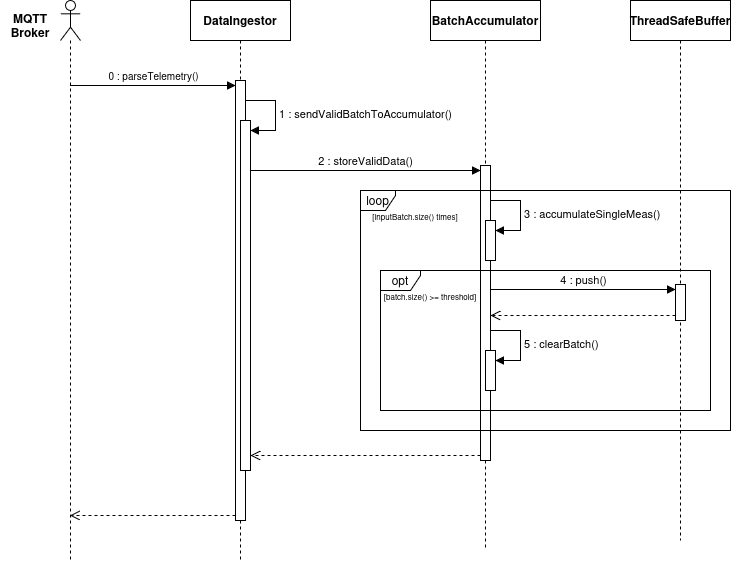
\includegraphics[width=\textwidth]{images/SequenceDiagram/Accumulation.drawio.png}
    \caption{AstraLog-HPC: Accumulation - Sequence Diagram}
    \label{fig:accumulation_dequence_diag}
\end{figure}

\subsubsection{Scenario 2: Rule Loading}
Before execution, the Rule Engine must load the rules required to evaluate data batches. The following scenario (\figurerefer{fig:ruleLoading_sequence_diag}) shows the pipeline:

\begin{figure}[htbp]
    \centering
    \label{fig:ruleLoading_sequence_diag}
    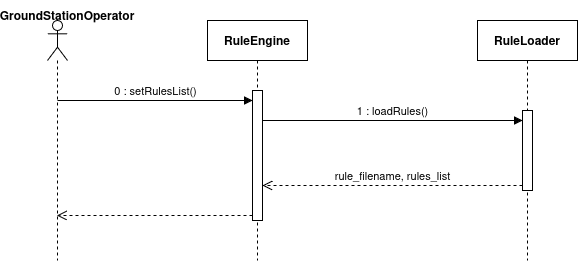
\includegraphics[width=\textwidth]{images/SequenceDiagram/RuleLoading.drawio.png}
    \caption{AstraLog-HPC: Rule Loading - Sequence Diagram}
    \label{fig:ruleLoading_sequence_diag}
\end{figure}

\subsubsection{Scenario 3: Rule Processing}
This scenario (\figurerefer{fig:ruleProcessing_sequence_diag}) shows how batches are processed from the queue.
\begin{itemize}
    \item \textbf{Retrieval and Evaluation:} The Rule Engine pops a batch from the ThreadSafeBuffer and evaluates it against configured rules, storing intermediate results in the MeasDatabase
    \item \textbf{Dispatch Routing:} After checking the rule outcomes, the engine routes the data to the OutputDispatcher. If all rules pass, valid data is appended; if any fail, alarms are dispatched instead.
    \item \textbf{Cleanup and Residuals}: Finally, the engine resets its cache and, if any residual data remains in the sub-batch, performs a final evaluation and storage pass.
\end{itemize}

\begin{figure}[htbp]
    \centering
    \label{fig:ruleProcessing_sequence_diag}
    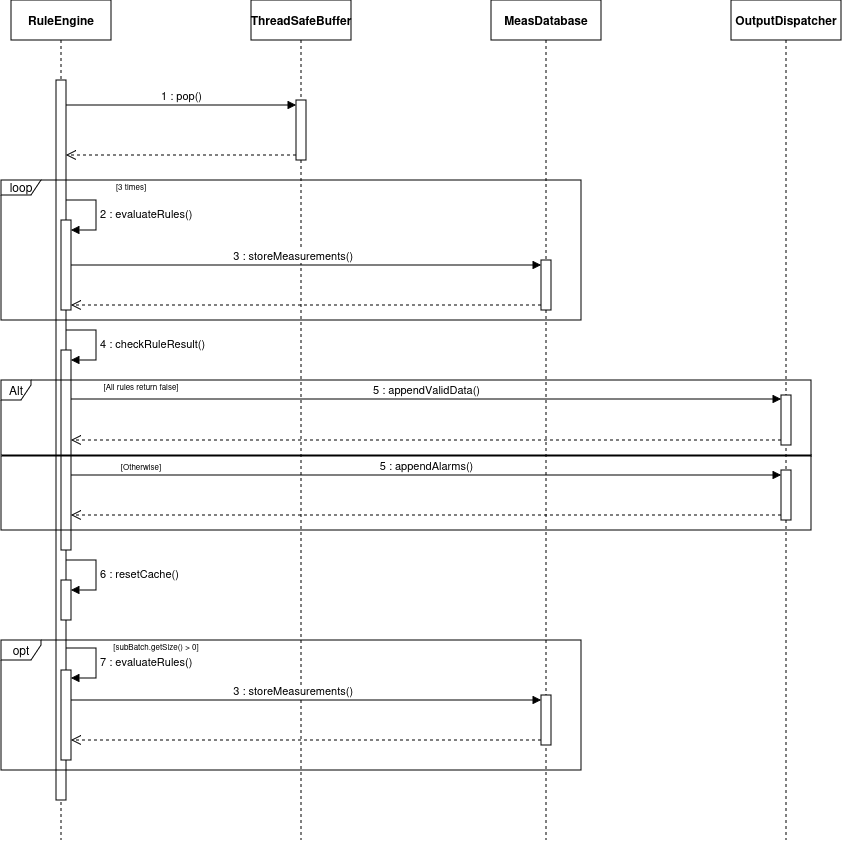
\includegraphics[width=\textwidth]{images/SequenceDiagram/RuleProcessing.drawio.png}
    \caption{AstraLog-HPC: Rule Processing - Sequence Diagram}
    \label{fig:ruleProcessing_sequence_diag}
\end{figure}

\clearpage
\subsection{Critical points and design decisions}
%TODO: Tell me what you think of this subdivision
\subsubsection{Architectural decisions}
The following decisions regard the choices made to ensure the AstraLog-HPC environment can handle continuous data telemetry while maintaining data integrity: 
\begin{itemize}
    \item The system adopts an Event-Driven Architecture \textbf{(EDA)} using a message broker in order to collect JSON packets coming from spacecraft's sensor. With this approach the system is able to manage the stream of data coming from the aircraft in an aynchronous way. The MQTT Broker topic acts as a collector guaranteeing zero data loss.
    \item The filtering of packets received by the system is performed with a parsing function inside the \textbf{DataIngestor} component that evaluates the correctness of JSON syntax.
    \item \textbf{Rule Engine} needs to maintain the state of previous measurements of sensors in order to check the validity of \textit{STATEFUL} rules. To do so, it is required a structure that acts as a memory and maps each \textit{sensor\_id} to the past measurements. This idea was later formalized into the MeasDatabase component.
    \item The design supports dual-mode operation: embedded execution for real time onboard ingestion and HPC cluster execution via SLURM for high-volume data anlysis. 
\end{itemize}

\subsubsection{Implementation and HPC integration}
The following points outline the technical strategies and patterns used to leverage High-Performance Computing capabilities for parallel data processing and efficient resource allocation:
\begin{itemize}
\item Data ingestion is managed via a Python script that utilizes a HiveMQ broker to receive a continuous data stream from an external academic website.
\item The system is implemented adopting the \textbf{C++} programming language to meet low-latency requirements and utilize high-quality, parallel JSON parsers.
\item To guarantee consistent deployment across the Cineca Galileo cluster, the application is containerised using Singularity, ensuring the execution environment does not vary from local testing to production cluster nodes.
\item The system generates standardised \verb|valid_data.csv| and \verb|alarms.log| according to the previously reported format, ensuring that all safety checks are human-readable and verifiable by mission personnel.  
\end{itemize}

\subsubsection{Quality assurance (CI/CD)}
To maintain the reliability and stability required for critical space mission software, the system incorporates automated workflows for continuous verification and validated output generation. In particular, the following strategies are adopted: 
\begin{itemize}
    \item A \textbf{CI/CD pipeline} is integrated via GitHub Actions, ensuring new software commit is automatically tested to verify stability and rule logic before deployment.

\end{itemize}

\clearpage
\section{Work distribution and effort}
The following table (\tablerefer{tab:work_distribution}) summarises the distribution of tasks for this document across team members and the estimated effort for each activity.
%TODO: This is kind of a mock: the timing is mostly fake as well as the names should better reflect how we divided the work. We shoul probably discuss this all together 
\begin{table}[h]
\label{tab:work_distribution_top}
\centering
\begin{tabularx}{\textwidth}{|X|X|c|c|}
\hline
\textbf{Task} & \textbf{Responsible} & \textbf{Effort (hours)} & \textbf{Status} \\
\hline
Requirements elicitation & Tobia Grimaldi, Dong Hua Zhu & 6 & Completed \\
\hline
Use case analysis & Tobia Grimaldi & 4 & Completed \\
\hline
Domain assumptions & Luca Salmoiraghi & 1 & Completed \\
\hline
Functional requirements & Luca Salmoiraghi, Tobia Grimaldi & 5 & Completed \\
\hline
Non-functional requirements & Luca Salmoiraghi, Tobia Grimaldi & 4 & Completed \\
\hline
Component Diagram & Luca Salmoiraghi, Dong Hua Zhu & 8 & Completed \\
\hline
Class Diagram & Dong Hua Zhu & 2 & Completed \\
\hline
Sequence Diagrams & Dong Hua Zhu & 8 & Completed \\
\hline
Critical points and decisions & Tobia Grimaldi & 1 & Completed \\
\hline
Document formatting \& LaTeX & Luca Salmoiraghi & 5 & Completed \\
\hline
AI tool integration \& disclosure & Luca Salmoiraghi, Dong Hua Zhu, \par Tobia Grimaldi & 1 & Completed \\
\hline
\textbf{Total} & & \textbf{45} & \\
\hline
\end{tabularx}
\caption{Work distribution and estimated effort}
\label{tab:work_distribution}
\end{table}

\clearpage
\section{On the usage of AI}
The following section details how Generative AI has been employed as a support tool for the project. In particular, the following actions have been AI-assisted: 
\begin{itemize}
    \item Grammatical review and general revision of sentence correctness (chatbot employed: DeepSeek);
    \item Title page styling (chatbot employed: Google Gemini), although it is to be noted that the final result is actually human-created with some suggestions integrated from the AI;
    \item Automation of table creation (chatbot employed: Google Gemini, DeepSeek), \LaTeX code was generated starting from a human-readable description of each table.
    \item Code refactoring (chatbots employed: Google Gemini and Claude): Generative AI was utilized to draft useless lines of code and troubleshoot compilation errors. All AI-generated snippets were subsequently reviewed, refactored, and tested.
    \item Test cases generation (chatbot employed: Gemini): AI tools helped with providing a right set of test cases that were used in order to assess the functionalities of the system.  
\end{itemize}

LLMs were largely used to review code quality and assist with architectural choices. These are some examples of the prompts used:

\begin{itemize}
    \item Is the function \verb|<function-name>| consistent? Please review its code quality and suggest improvements.
    \item What is the most efficient way to use MPI communicators for this specific function?
    \item Can you review this c++ code and tell if its structure is correct?
\end{itemize}

We used AI to accelerate testing and performance assessment. Some scripts where used to generate deterministic rules and test scenarios.

In particular, we used AI models (\texttt{Gemini}, \texttt{Claude}) to generate scripts that tested our model parallelisation performance. This allowed rapid and repeatable comparisons between the OpenMP and OpenMP+MPI variants and helped identify that MPI communication overhead dominated the execution time. AI-driven test generation and result aggregation significantly sped up our benchmarking iterations.

\begin{itemize}
    \item Generate a script in c++ that tests the parallelization workflow. I want a deterministic set of rules and measurements that the system has to evaluate with both OpenMP and OpenMPI+OpenMP application. 
    
    Provide also a bash script I can use to test different OpenMPI parallel distributions. Append the results in a .csv file.
\end{itemize}

In addition to that, AI was largely used in order to understand the constraints of Galileo100 cluster architecture. With the joint usage of Cineca's documentations and LLM we were able to figure out a CD pipeline able to deploy the application on an HPC environment with many limitations. Some examples:

\begin{itemize}
    \item How can I configure a CI/CD pull-based workflow on the Galileo100 cluster?
    \item Is Galileo100 cluster allowing api calls to the Github API?
    \item Is it possible to run consecutive slurm jobs after a certain period of time given the cluster's crontab limitations?
\end{itemize}

\end{document}